
\section{NEFD Method 3: dependencies on the observed opacity {\color{blue} Juan$\&$Laurence}}
\label{NEFD_pipeline}

In this section we investigate the astronomer NEFD as a function of
the atmospheric opacity and air mass.            
The date sets include all the scans that met the baseline section
criteria of Sect.~\ref{se:baseline_selection} and for which the flux
density estimates do not exceed $1~\rm{Jy}$. Indeed we show that the
measured NEFD from scans of sources brighter than $1~\rm{Jy}$ are
biased toward high values due to source signal leakage into the noise
estimates.

\addparag{ Flux cut + Fig. NEFD vs Flux JUAN} 


\begin{figure}
\begin{center}
 %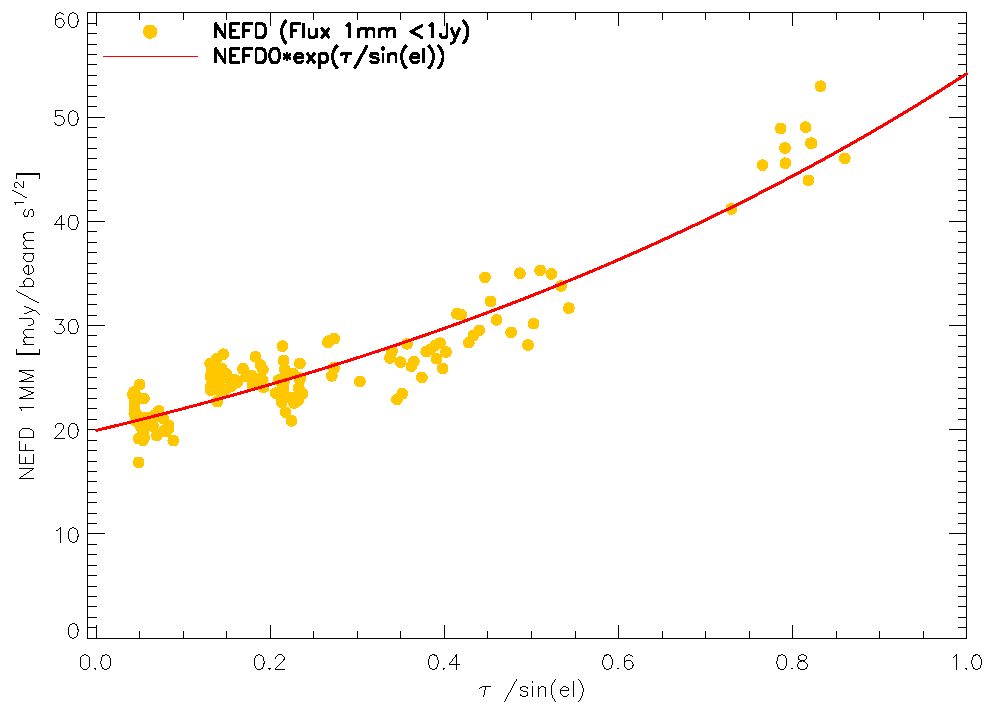
\includegraphics[clip, angle=0, scale=0.8]{Figures/NEFDIndScans/nefd_1mm_R9_F1_tau_run22_23.pdf}
 %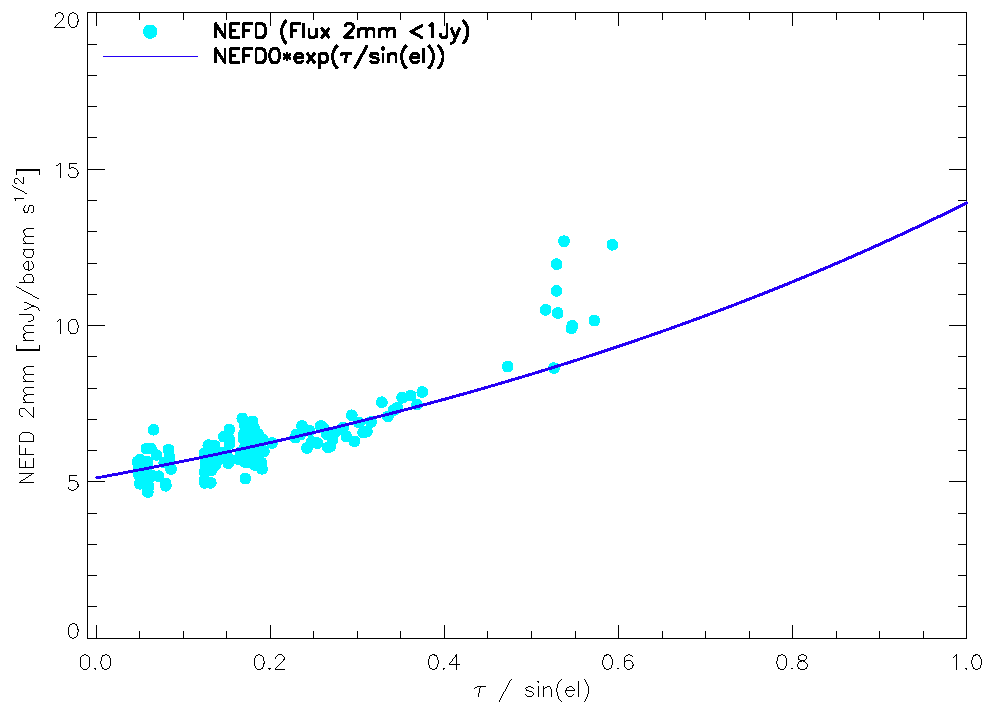
\includegraphics[clip, angle=0, scale=0.8]{Figures/NEFDIndScans/nefd_2mm_R9_F1_tau_run22_23.pdf}
 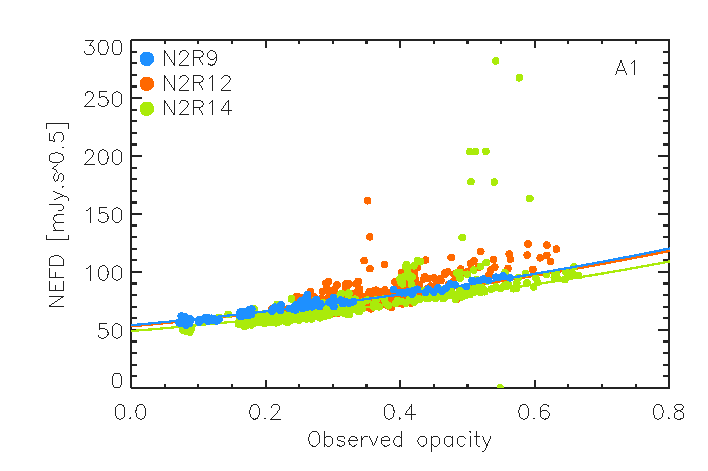
\includegraphics[clip=true,width=0.47\textwidth]{Figures/NEFD/plot_nefd_vs_obstau_a1.pdf}
 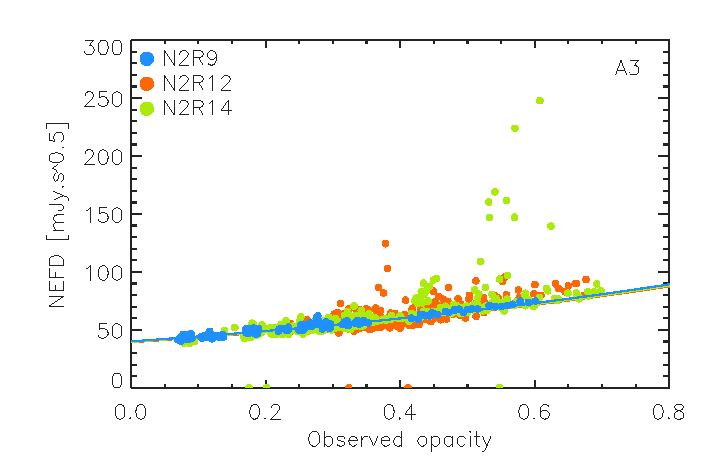
\includegraphics[clip=true,width=0.47\textwidth]{Figures/NEFD/plot_nefd_vs_obstau_a3.pdf}
 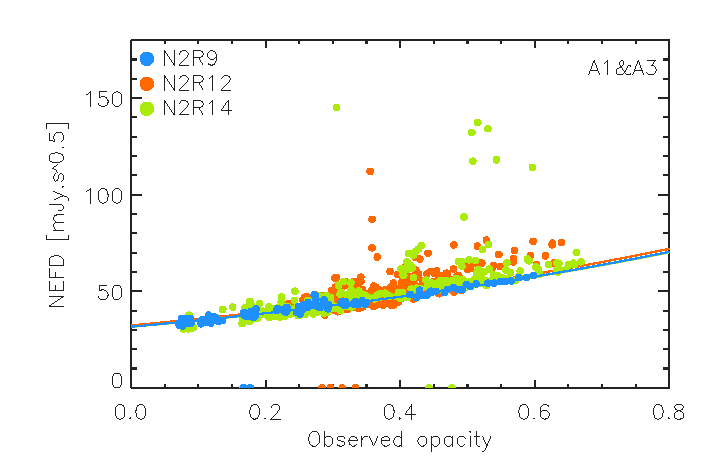
\includegraphics[clip=true,width=0.47\textwidth]{Figures/NEFD/plot_nefd_vs_obstau_1mm.pdf}
 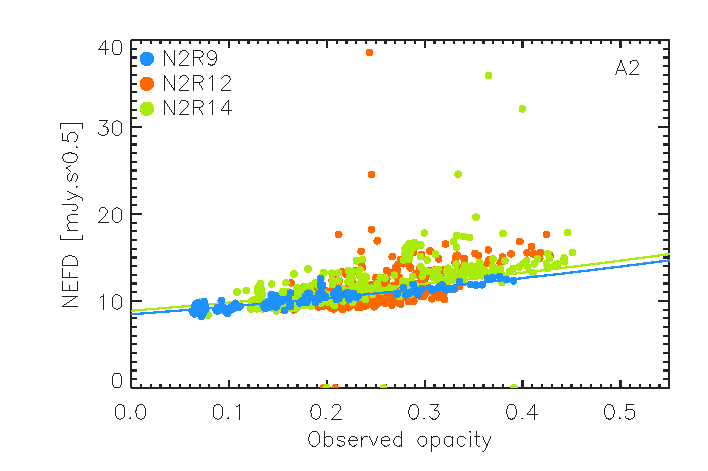
\includegraphics[clip=true,width=0.47\textwidth]{Figures/NEFD/plot_nefd_vs_obstau_a2.pdf}
 \caption[Measured NEFD versus observed opacity]{Measured NEFD as a function of atmospheric background for array 1 (upper left), array 3 (upper right), the $1~\rm{mm}$ (lower left) and $2~\rm{mm}$ (lower right) channels. Datapoints are NEFD estimates in $\rm{mJy}\cdot s^{0.5}$ for N2R9 (blue), N2R12 (orange) and N2R14 (chartreuse). We also show in the plots the expected NEFD evolution with atmospheric background as solid curves.}
\label{fig:nefdvsbackground}
\end{center}
\end{figure}
 
%% \subsection{NEFD Method 3: scan NEFD vs opacity and air mass}
%% \begin{figure}
%% \begin{center}
%% 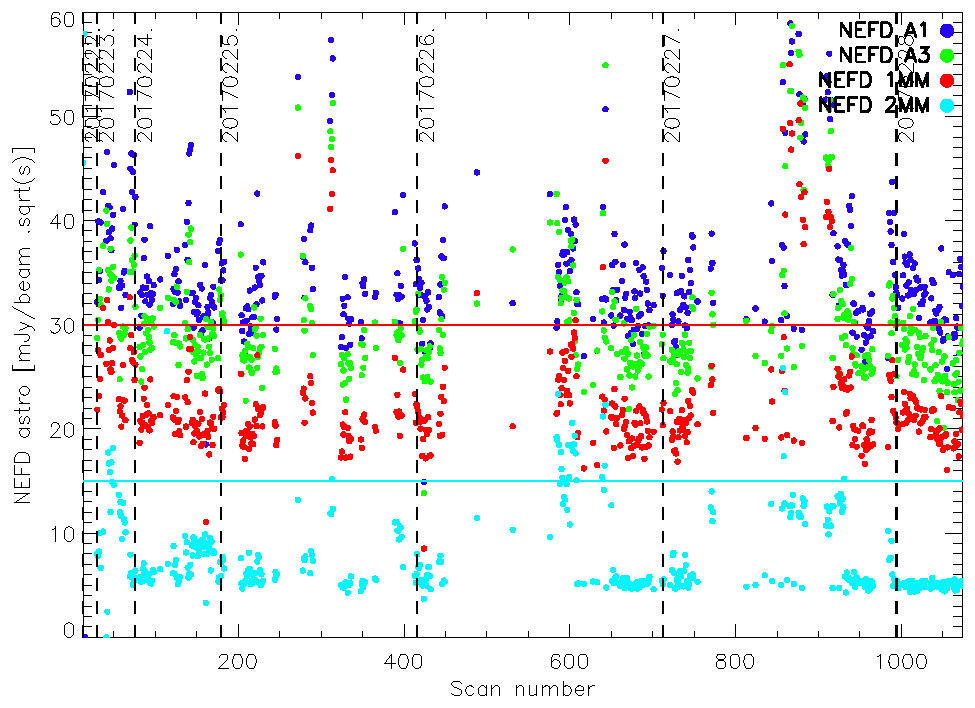
\includegraphics[clip, angle=0, scale =0.8]{Figures/NEFDIndScans/nefd_evol_run22.pdf}
%% \caption{Evolution of the measured instrument NEFD across scans for N2R9.}
%% \label{fig:nefdvsscans}
%% \end{center}
%% \end{figure}
%% 
%% \begin{figure}
%% \begin{center}
%% 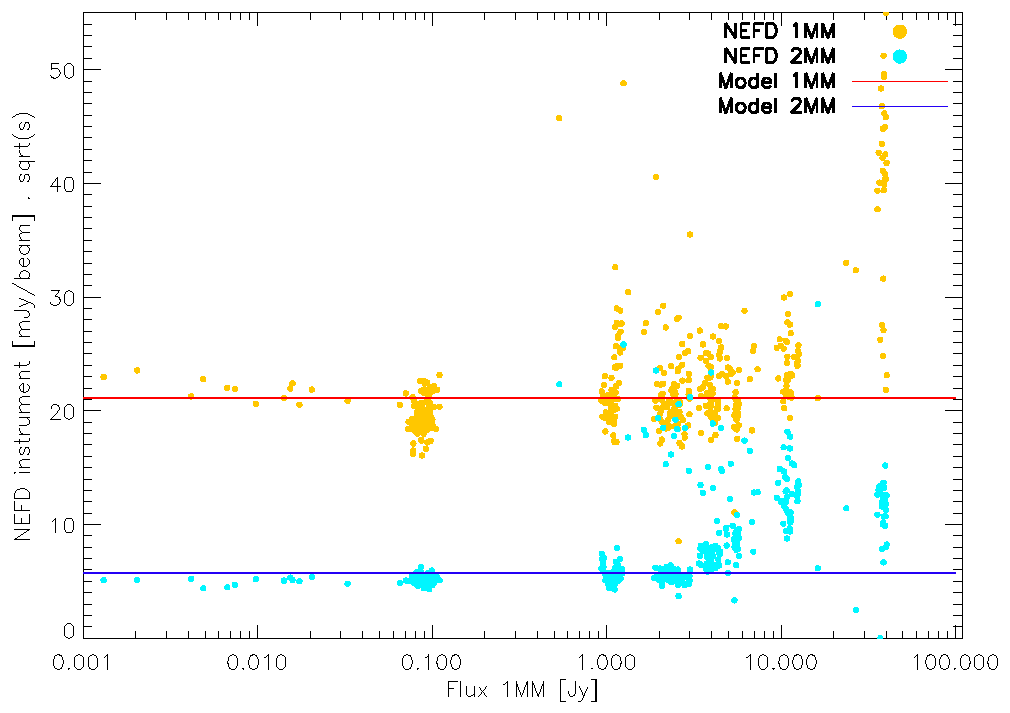
\includegraphics[clip, angle=0, scale =0.8]{Figures/NEFDIndScans/nefd_flux1mm_run22.pdf}
%% \caption{Measured instrument NEFD as a function of the flux of the source.}
%% \label{fig:nefdvsflux}
%% \end{center}
%% \end{figure}
%% \begin{figure}
%% \begin{center}
%% 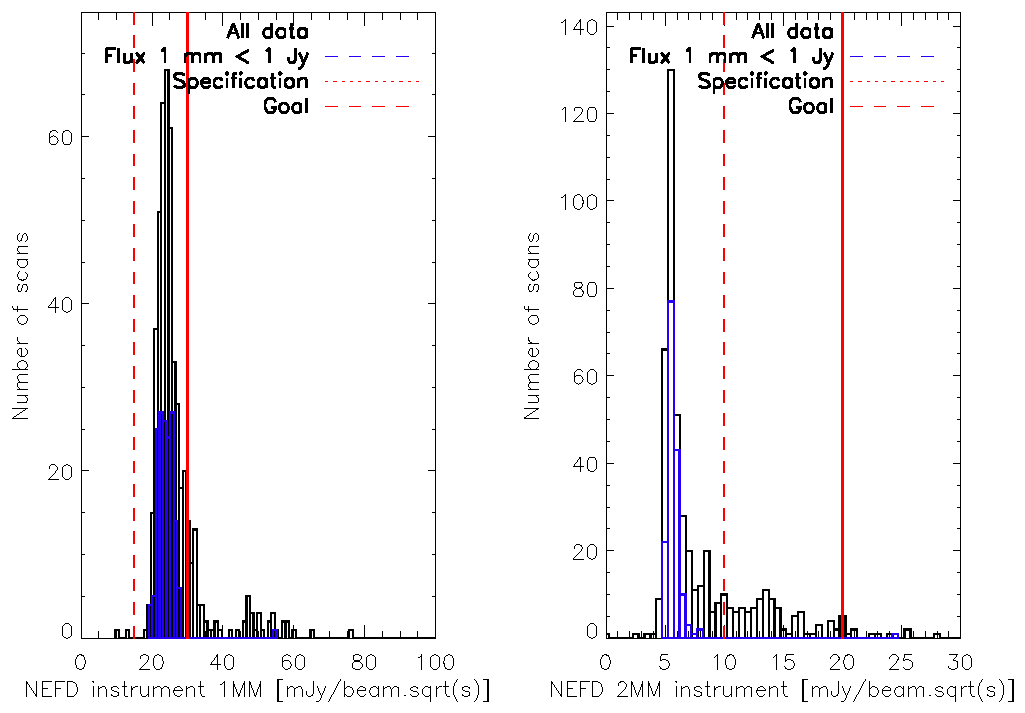
\includegraphics[clip, angle=0, scale =0.8]{Figures/NEFDIndScans/hist_nefd_ref_run22.pdf}
%% \caption{Histogram of the measured reference NEFD across the N2R9 for the 1 (right) and 2 (left) mm channels.}
%% \label{fig:nefdhist}
%% \end{center}
%% \end{figure}
%%  
%%

 Figure~\ref{fig:nefdvsbackground} shows the
 measured NEFD, which we refer to as astronomer NEFD, for the 1 and 2 mm as a
 function of the measured atmospheric background in terms of $\tau/sin(El)$. The
 atmospheric opacity was computed as discussed in Section~\ref{se:opacities}. We
 observe that the increase of the astronomer NEFD is in agreement with what we
 would expect for background dominated sensitivity.

Baseline astromoner and instrument NEFD results are gathered in
Table.~\ref{tab:baseline_nefd_pipeline}.

\begin{table}
\begin{center}
\begin{tabular}{|c|c|rrrr|}
\hline
NEFD type & Arrays & N2R9 & N2R12 & N2R14 & Combined  \\
\hline\hline
Astronomer  & A1       &  64.8 & 63.6 &  58.7 &  62.7 \\
            & A3       &  48.3 & 47.3 &  47.7 &  47.7 \\ 
            & A1 \& A3 &  38.0 & 38.9 &  37.9 &  38.3 \\
            & A2       &   9.4 &  9.4 &   9.8 &   9.5  \\
\hline
Instrument  & A1       &   54.0 & 53.1 &  49.0 & 52.3  \\
            & A3       &   40.1 & 39.3 &  39.6 & 39.6  \\ 
            & A1 \& A3 &   31.6 & 32.3 &  31.5 & 31.9  \\
            & A2       &    8.5 &  8.5 &  8.9  &  8.6  \\
\hline\hline
\end{tabular}
\label{tab:baseline_nefd_pipeline}
\caption[NEFD using method 3]{Astromoner (average IRAM observing conditions) and Instrument (zero opacity) NEFD estimates in mJ.s$^{0.5}$ for N2R9, N2R12 and N2R14 campaigns and for the union of the observations acquired during the three campaigns, that are more than a thousand scans. }
\end{center}
\end{table}



 %We observe however some
 %significant deviations from the curve. To investigate this issue we also show in
 %Figure~\ref{fig:nefdvsscans} the evolution of the background corrected NEFD,
 %hereafter instrument NEFD, across the N2R9 campaign for arrays A1 (blue), A3
 %(green) and A2 (cyan), and for the combination of A1 and A3 (red). We globally
 %observe stable NEFD across the run, with A1 sensitivity being worse than for
 %A3. We also show the measured instrument NEFD as a function of the flux of the
 %source in the 1 mm channel in Figure~\ref{fig:nefdvsflux}. We observe that the
 %observed deviations in the instrument NEFD correspond mainly to the large flux
 %source scans. This is more obvious in Figure~\ref{fig:nefdhist} where we present
 %the histogram of the measured NEFD for 2 mm of pwv and at a elevation of 60
 %degrees, hereafter, reference NEFD, for the 1 and 2 mm channels.


